\documentclass{beamer} \usetheme{Madrid}
\usecolortheme{beaver}

\setbeamertemplate{enumerate items}[circle]
\setbeamercolor{item projected}{bg=red!70!black}

\usepackage[utf8]{inputenc}
\usepackage{mdframed}
\usepackage{minted}
\usepackage{tikz}
\usetikzlibrary{automata, positioning, arrows}

\tikzset{
    ->,
    node distance=3cm,
    every state/.style={thick, fill=gray!10},
    initial text=$ $,
}

\newenvironment{question}[1][]{
    \ifstrempty{#1}{}
    {\mdfsetup{
        frametitle={
            \tikz[baseline=(current bounding box.east),outer sep=0pt]
            \node[anchor=east,rectangle,fill=gray!30]
            {#1};
        }
    }}
    \mdfsetup{
        innertopmargin=10pt,linecolor=gray!30,
        linewidth=2pt,topline=true,
        frametitleaboveskip=\dimexpr - \ht\strutbox\relax
    }
    \begin{mdframed}
}{
    \end{mdframed}
}

\title{Git Workshop}
\subtitle{Fall 2020}

\author[]{Jack Leightcap\inst{1}\inst{2} \and Connor Northway\inst{2}}

\institute[IEEE, Wireless Club]{
    \inst{1}IEEE -- \url{nuieeeofficers@gmail.com}
    \and
    \inst{2}Wireless Club -- \url{nuwirelessclub@gmail.com}
}

\date[Fall 2020]{December 7, 2020}

\begin{document}
\frame{\titlepage}

\begin{frame}
    \frametitle{Intro: Workshop Structure}
    \centering \textbf{Structure:}
    \begin{enumerate}
        \setlength\itemsep{1em}
        \item Talk: how does \texttt{Git} work?
        \item Example: managing homework
        \item Hands-on: solve \texttt{Git} `puzzles' in browser
    \end{enumerate}
    \vfill
    \centering \textbf{General:}
    \begin{itemize}
        \setlength\itemsep{1em}
        \item Ask questions!
              (want to know more? something isn't clear?)
        \item Reach out: \url{neuwireless.slack.com}
    \end{itemize}
\end{frame}

\begin{frame}
    \frametitle{Background: What is \texttt{Git}?}
    \vfill
    \begin{figure}
        
\includegraphics[height=15mm]{logo.png}
        \caption{Git Logo --- CC BY 3.0}
    \end{figure}
    \vfill
    \begin{itemize}
        \item broadly; \emph{a tool used to track changes to files and folders.}
        \item facilitates collaboration on software projects
        \item captures `snapshots' of a project
        \item maintains metadata
        \begin{itemize}
            \item what was changed
            \item who was it changed by
            \item when was it changed
            \item messages associated with changes
        \end{itemize}
    \end{itemize}
    \vfill
\end{frame}

\begin{frame}
    \frametitle{Background: What is \texttt{Git} used for?}
    \vfill
    \centering \textbf{Group Applications (Industry, co-op)}
    \begin{itemize}
        \item large software projects
        \item resolve conflicts when multiple people are editing the same things
        \item who wrote this!?
    \end{itemize}
    \vfill
    \centering \textbf{Personal Applications}
    \begin{itemize}
        \item ``I swear this worked 10 minutes ago\ldots''
        \item find what broke something and when
        \item separate tasks; work on bug fixing is isolated from work on new feature
        \item can use for class work!
    \end{itemize}
    \vfill
\end{frame}

\begin{frame}
    \frametitle{Background: Big Idea of \texttt{Git}}
    \begin{question}[QUESTION: Intuition]
        based on this description of what \texttt{Git} does, can you imagine how you would go about making these `snapshots' manually?
    \end{question}
    \vfill
    \begin{figure}
        
\includegraphics[width=3cm]{final.png}
    \end{figure}
\end{frame}

\begin{frame}
    \frametitle{Background: Big Idea of \texttt{Git}}
    \begin{center}
        \begin{figure}
            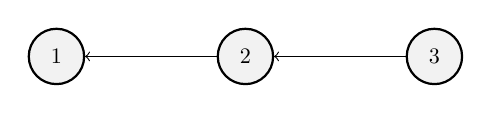
\begin{tikzpicture}[scale=0.8, every node/.style={transform shape}]
                \node[state] (q1) {1};
                \node[state, right of=q1] (q2) {2};
                \node[state, right of=q2] (q3) {3};

                \draw (q2) edge node{} (q1)
                      (q3) edge node{} (q2)
                ;
            \end{tikzpicture}
            \caption{Linear History}
        \end{figure}
        \vfill
        \begin{figure}
            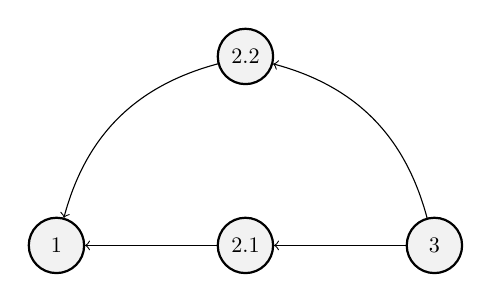
\begin{tikzpicture}[scale=0.8, every node/.style={transform shape}]
                \node[state] (q1) {1};
                \node[state, right of=q1] (q21) {2.1};
                \node[state, above of=q21] (q22) {2.2};
                \node[state, right of=q21] (q3) {3};

                \draw (q21)  edge node{} (q1)
                      (q22)  edge[bend right] node{} (q1)
                      (q3) edge node{} (q21)
                      (q3) edge[bend right] node{} (q22)
                ;
            \end{tikzpicture}
            \caption{Branched History}
        \end{figure}
    \end{center}
\end{frame}

\begin{frame}
    \frametitle{Example: Managing Local Files}
    \vfill
    \begin{question}[EXAMPLE: Homework Files]
        \begin{enumerate}
            \item \emph{Init}: make some files, `save' them
            \item \emph{Commit}: changes, save those as well
            \item \emph{Checkout/Restore}: whoops, deleted something, restore it
            \item \emph{Branch}: new feature, make a new branch
            \item \emph{Merge}: done, merge back
        \end{enumerate}
    \end{question}
    \vfill
\end{frame}

\begin{frame}
    \begin{figure}
        
\includegraphics[height=\textheight-2cm]{xkcd.png}
        \caption{XKCD 1597 `Git' --- CC BY-NC 2.5}
    \end{figure}
\end{frame}

\begin{frame}
    \frametitle{See Also}
    \begin{itemize}
        \item \url{https://wyag.thb.lt/} -- implement git from scratch in Python
    \end{itemize}
\end{frame}

\end{document}
